\begin{figure*}[thb!]
  \centering
  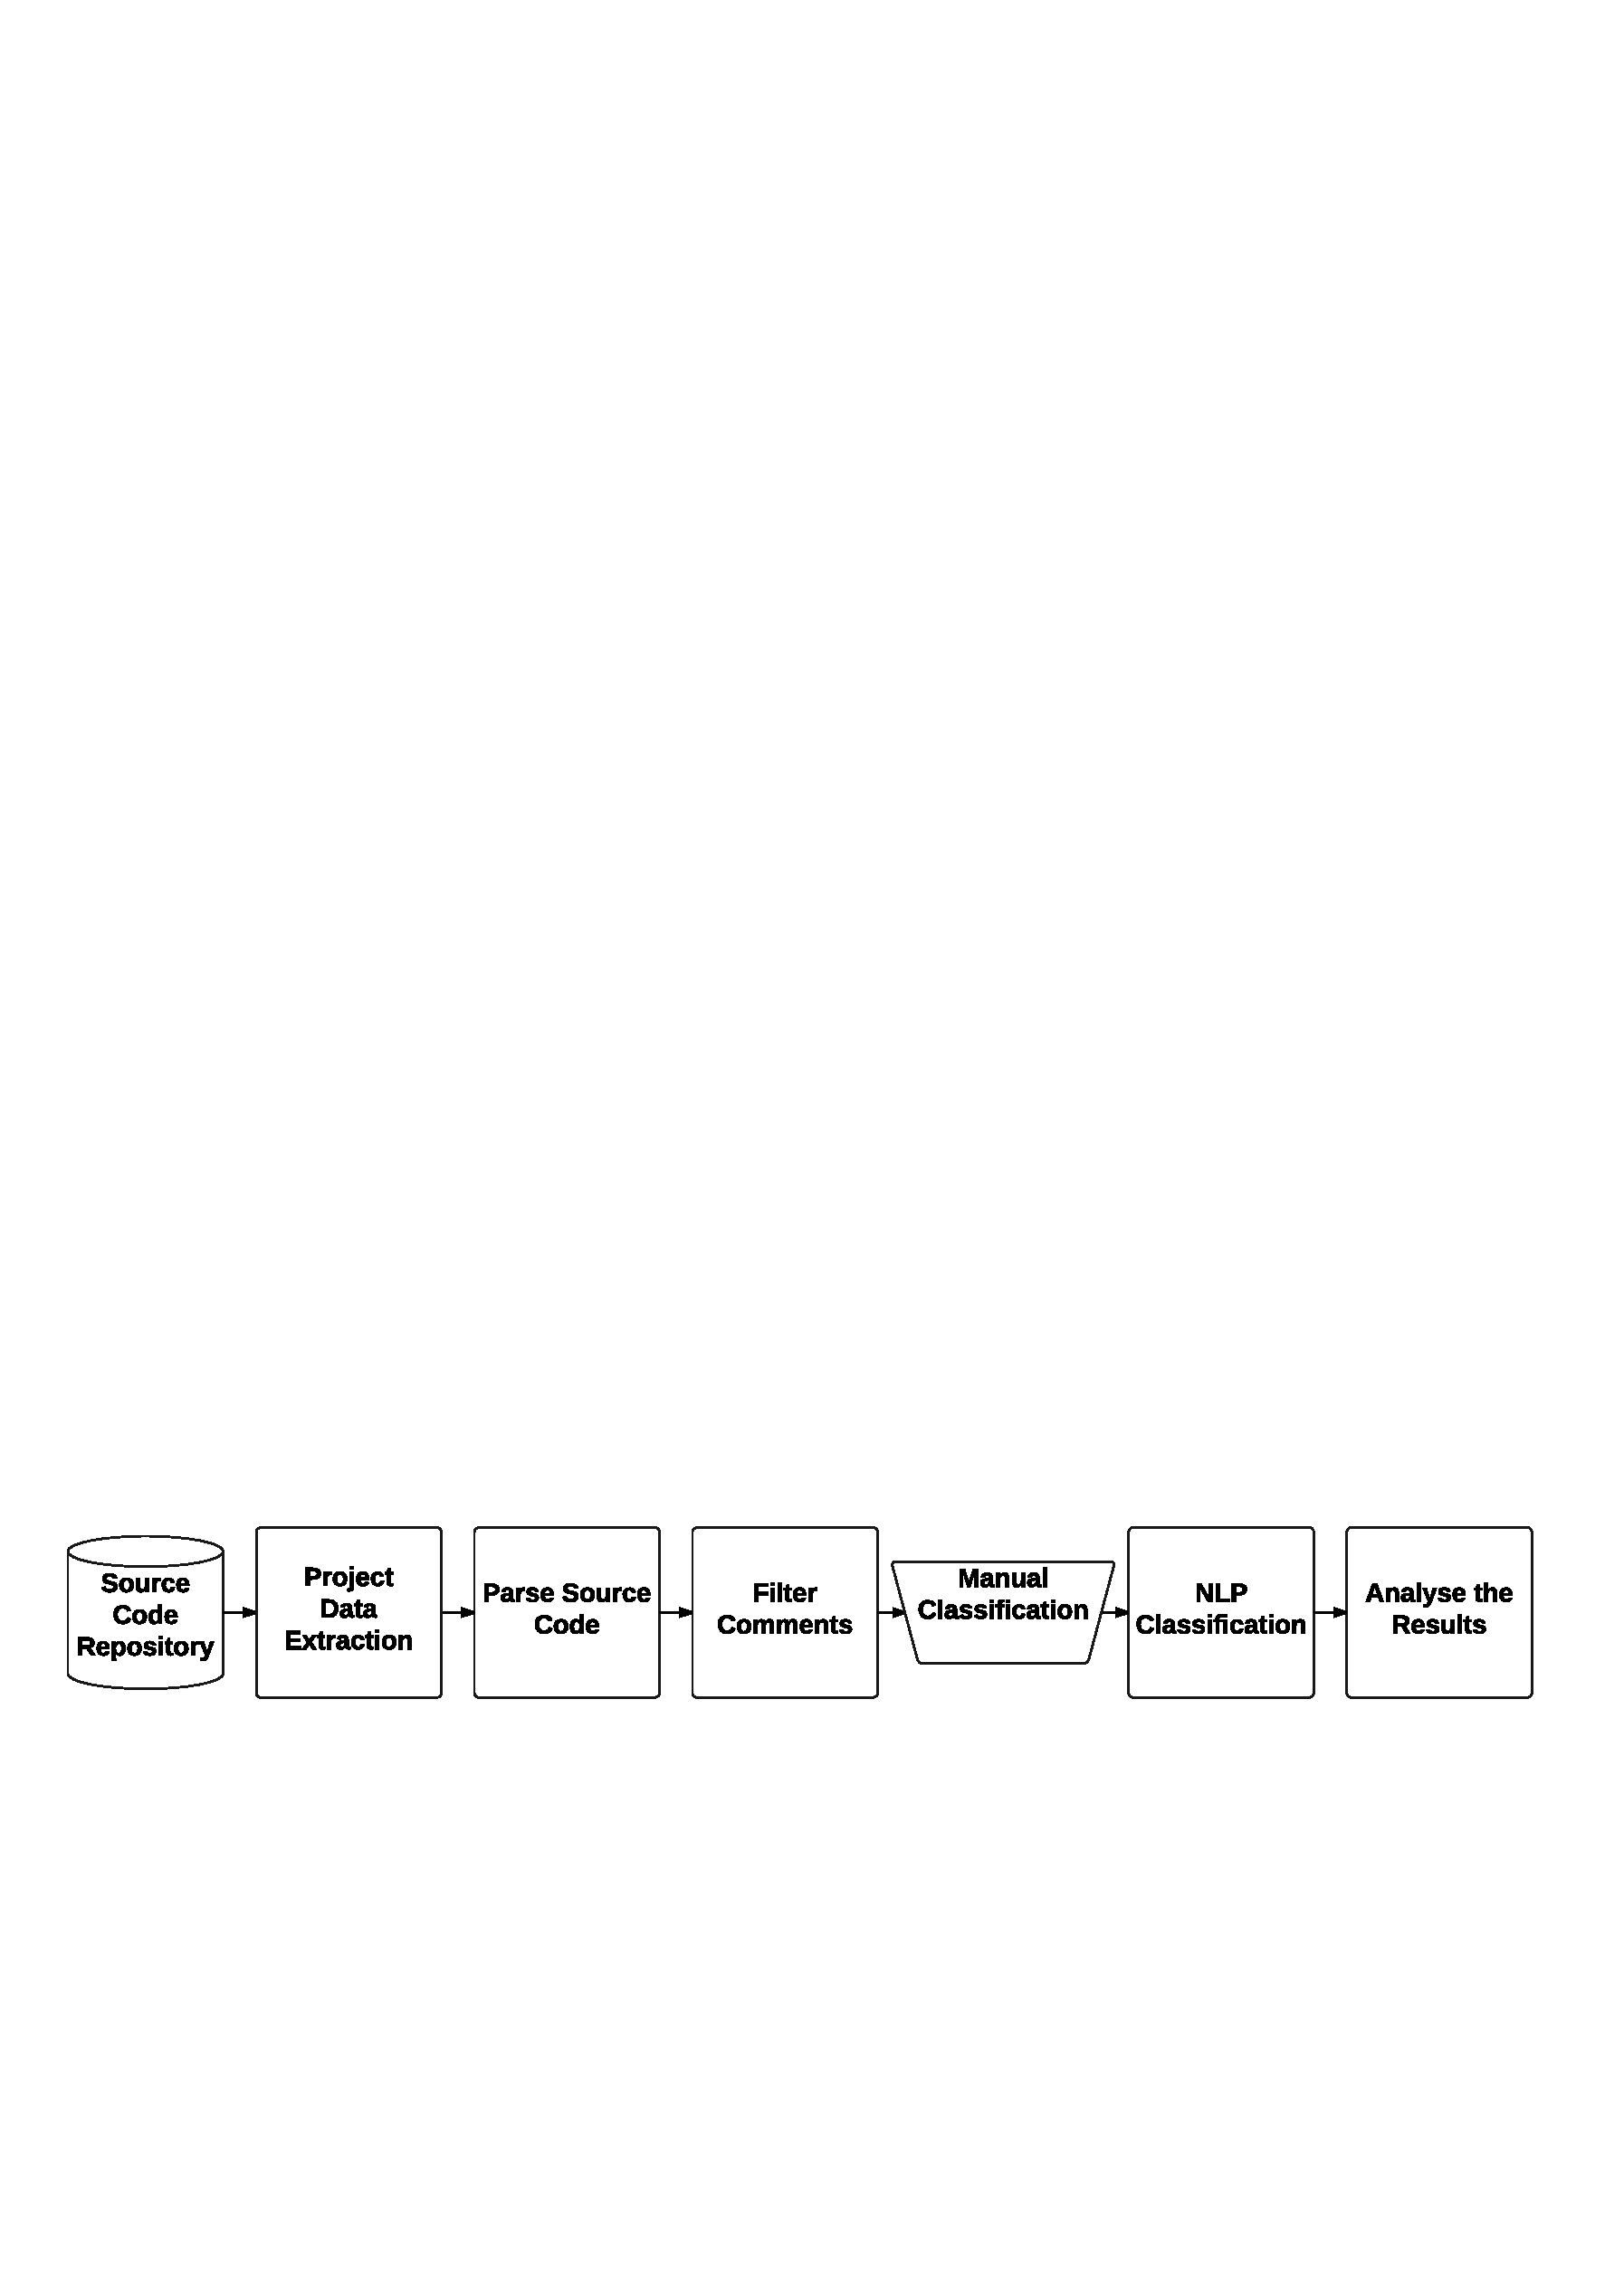
\includegraphics[width=1\textwidth]{figures/approach.pdf}
  \caption{Approach overview}
  \label{fig:approach}
\end{figure*}

The main goal of our study is to automatically identify \SATD through source code comments. To do that, we first extract the comments from ten open source projects. Second, we apply four filtering heuristics to remove comments that are irrelevant for the identification of \SATD  (e.g., license comments, commented source code and Javadoc comments). After that, we manually classify the remaining comments into \SATD types (i.e., design debt, requirement debt, defect debt, documentation debt and test debt). Lastly, we use these comments as training data to the Stanford  Classifier. Figure~\ref{fig:approach} shows an overview of our approach, and the following subsections details each step.

\subsection{Project Data Extraction} % (fold)
\label{sub:data_extraction}

To perform our study, we extract the source code of ten open source projects, namely Ant, Apache Jmeter, ArgoUML, Columba, EMF, Hibernate, JEdit, JFreeChart, JRuby and SQuirrel. We selected these projects since they belong to different application domains, and vary in size (e.g., SLOC), and in the number of contributors. 

Table \ref{tab:project_details} provides more information about each one of the projects used in our study, listed in the first column. The second column provides the release used, followed by the number of classes, the total source lines of code (SLOC), the number of contributors, the total extracted comments, the number of comments analyzed after applying our filtering heuristics, the number of comments that were classified as \SATD, the percentage of these comments that represent design debt, the percentage of \SATD comments classified as requirement debt and finally the percentage of all other types of debt (i.e., defect, documentation and test debt). 

Since there are many different definitions for the SLOC metric we clarify that, in our study, a source line of code contains at least one valid character, which is not a blank space or a source code comment. In addition, we only use the Java files to calculate the SLOC, and to do so, we use the tool SLOCCount \cite{wheeler2004:home}. 

The number of contributors was extracted from OpenHub, an on-line community and public directory that offers analytics, search services and tools for open source software \cite{Openhub:home}. It is important to notice that the number of comments shown for each project does not represent the number of commented lines, but rather the number of individual line, block, and Javadoc comments. 

In total, we obtained 259,229 comments, found in 16,249 Java classes. The size of the selected projects varies between 81,307 and 228,191 SLOC's, and the number of contributors of these projects ranges from 9 to 326. 

\begin{table*}[thb!]
    \begin{center}
    \caption{Project Details}
    \label{tab:project_details}
            \begin{tabular}{l| c c r c c c c c c c}
            \toprule
            \thead{Project}   & \thead{Release}  & \thead{\# of \\classes}   & \thead{SLOC} & \thead{\# of \\contributors}  & \thead{\# of \\comments}   & \thead{\# of \\comments \\after filtering} & \thead{\# of \\TD \\comments} & \thead{\% of \\Design \\Debt} & \thead{\% of \\Requirement \\Debt} & \thead{\% of \\Other \\Debts}\\ 
            \midrule 
            Ant            & 1.7.0    & 1,475 & 115,881 & 74  & 21,587 &   4,137 &    131 &  72.51  & 09.92  & 17.55 \\
            ArgoUML        & 0.34     & 2,609 & 176,839 & 87  & 67,716 &   9,548 &  1,413 &  56.68  & 29.08  & 14.22 \\
            Columba        & 1.4      & 1,711 & 100,200 & 9   & 33,895 &   6,478 &    204 &  61.76  & 21.07  & 17.15 \\
            EMF            & 2.4.1    & 1,458 & 228,191 & 30  & 25,229 &   4,401 &    104 &  75.00  & 15.38  & 09.61 \\
            Hibernate      & 3.3.2 GA & 1,356 & 173,467 & 226 & 11,630 &   2,968 &    472 &  75.21  & 13.55  & 11.22 \\
            JEdit          & 4.2      &   800 &  88,583 & 57  & 16,991 &  10,322 &    256 &  76.56  & 05.46  & 17.96 \\
            JFreeChart     & 1.0.19   & 1,065 & 132,296 & 19  & 23,474 &   4,423 &    209 &  88.03  & 07.17  & 04.78 \\
            Jmeter         & 2.10     & 1,181 &  81,307 & 33  & 20,084 &   8,162 &    374 &  84.49  & 05.61  & 09.89 \\
            JRuby          & 1.4.0    & 1,486 & 150,060 & 328 & 11,149 &   4,897 &    622 &  55.14  & 17.68  & 27.17 \\ 
            SQuirrel       & 3.0.3    & 3,108 & 215,234 & 46  & 27,474 &   7,230 &    286 &  73.07  & 17.48  & 09.44 \\ 
            \bottomrule             
        \end{tabular}
    \end{center}
\end{table*}


% subsection data_extraction (end)
\subsection{Parse Source Code} % (fold)
\label{sub:parse_source_code}

After obtaining the source code of all projects, we extract the comments from the source code. We use JDeodorant \cite{Tsantalis2008CSMR}, an open-source Eclipse plug-in, to parse the source code and extract the code comments. JDeodrant uses the Eclipse AST framework to create an Abstract Syntax Tree (AST) map of the source code. The AST map contains detailed information about the project such as: the source code comments, its type (i.e., Block, Single-line or Javadoc) and the line where each one of these comments starts and ends. 

Due to these features, we adapted JDeodorant to extract the aforementioned information about source code comments and store it in a relational database to facilitate the processing of the data.

% subsection parse_source_code (end)
\subsection{Filter Comments} % (fold)
\label{sub:filter_comments}

Source code comments can be used for different purposes in a project such as giving context, as part of the documentation, to express thoughts, opinions and authorship, and in some cases, to remove source code from the program. Comments are used freely for developers and with limited formalities, if any at all. This informal environment allows developers to bring to light opinions, insights and even confessions (e.g., self-admitted technical debt). 

As shown in prior work by Potdar and Shihab \cite{Potdar2014ICSME}, part of these comments can be identified as self-admitted technical debt, but they are not the majority of cases. With that in mind, we develop and apply 5 filtering heuristics to narrow down the comments eliminating the ones that are less likely to be classified as self-admitted technical debt.

To do so, we developed a Java based tool that reads from the database the data obtained by parsing the source code. Next, it executes the filtering heuristics and stores the results back in the database. The retrieved data contains information like the line number that a class/comment begins/ends and the type, considering the Java syntax, of the comment (i.e., Block, Single-line or Javadoc). With this information we process the filtering heuristics as described next.

License comments are not very likely to contain self-admitted technical debt, and are commonly added before the declaration of the class. We create a heuristic that removes comments that are placed before the class declaration. Since we know the line number that the class was declared we can easily check for comments that are placed before that line and remove them. In order to decrease the chances of removing a self-admitted technical debt comment while executing this filter we calibrated this heuristic to not remove comments containing one of task-reserved words (i.e., ``todo'', ``fixme'', or ``xxx'') ~\cite{Storey2008ICSE}.

Long comments that are created using multiple \emph{Single-line} comments instead of a \emph{Block} comment can hinder the understanding of the message considering the case that the reader (i.e., human or machine) analyzes each one of these comments independently. To solve that problem, we create a heuristic that searches for consecutive Single-line comments and groups them as one. We identify consecutive comments by subtracting the line number of both comments. For example, Single-line comment A is placed in line number 100 and Single-line comment B is placed in line 101. The subtraction of the line numbers will result in -1, therefore the comments are consecutive.
 
Commented source code is found in the projects due to many different reasons. One of the possibilities is that the code is not currently being used. Other is that, the code is used for debugging purposes only. Based on our analysis, commented source code does not have self-admitted technical debt. Our heuristic removes commented source code using a simple regular expression that captures typical Java code structures.

Comments that are automatically generated by the IDE were filtered as well. These comments are inserted as part of code snippets used to create constructors, methods and try catch blocks, and have fixed format (i.e., ``Auto-generated constructor stub'', ``Auto-generated method stub'' and ``Auto-generated catch block''). Therefore our heuristic search for these comments containing these patterns and remove them. 

Javadoc comments rarely mention self-admitted technical debt. For the Javadoc comments that do mention self-admitted technical debt, we notice that they usually contain one of the task-reserved words (i.e., ``todo'', ``fixme'', or ``xxx''). Therefore, our heuristic removes all comments of the type Javadoc unless they contain at least one of the task-reserved words. To do so, we create a simple regular expression that search for the task-reserved words before removing the comment.  

The steps mentioned above significantly reduced the number of comments in our dataset and helped us focus on the most applicable and insightful comments. For example, in the Ant project, applying the above steps helped to reduce the number of comments from 21,587 to 4,137 meaning a reduction of 80.83\% in the number of comments to be manually analyzed. Using the filtering heuristics we were able to remove from 39.25\% to 85.89\% of all comments. Table \ref{tab:project_details} provides the number of comments kept after the filtering heuristics for each project.

% subsection filtering_comments (end)

\subsection{Manual Classification} % (fold)
\label{sub:manual_classification}

Our goal is to inspect each comment and attribute to it the suitable technical debt classification. Since there are many comments, we developed a Java based tool that shows one comment at a time and gives a list of possible classifications that can be manually assigned to the comment. The list of possible classifications is based on previous work by Alves \textit{et al.}~\cite{Alves2014MTD}. In their work, a ontology on technical debt terms was proposed, and they identified the following types of technical debt across the researched literature: architecture, build, code, defect, design, documentation, infrastructure, people, process, requirement, service, test automation and test debt. 

During the classification process we notice that not all types of debt mentioned in \cite{Alves2014MTD} could be found in code comments. However, we were able to identify the following types of debt in the source comments: design debt, defect debt, documentation debt, requirement debt and test debt.

In our previous work ~\cite{Maldonado2015MTD} we manually classified 33,093 comments, and in the current study we manually classified 29,473 more comments. Which means that we extended our classified comments dataset in 89.06\%. In total, we manually classified 62,566 comments into the five different types of self-admitted technical debt mentioned above. The classification process took approximately 185 hours in total, and was performed by the first author of the paper. 

% We manually classified 63,015 comments into different types of self-admitted technical debt. During the classification process we notice that not all types of debt mentioned in \cite{Alves2014MTD} could be found in code comments. However, we were able to identify the following types of debt in the source comments: design debt, defect debt, documentation debt, requirement debt and test debt. The classification took approximately 185 hours and was performed by the first author of the paper. 

It is very important to clarify that this manual classification step does not need to be repeated in order to apply our approach since our dataset is public available.   

To mitigate the risk of creating a dataset too biased we created a statistically significant sample of our dataset and asked for a master student to classify it. To prepare the student for the task we gave an 1 hour explanation about the different kinds of \SATD, and walked the student through a couple of examples of each different type of \SATD comment. 

The statistically significant sample was created based on the total number of comments (62,566) with a confidence level of 99\% and a confidence interval of 5\%. Resulting in a stratified sample of 659 comments. We composed the stratified sample accordingly with the percentage of each classification found in the original dataset. Therefore, the stratified sample was composed of: 92\% of comments with no \SATD (609 comments), 4\% of design debt comments (29 comments), 2\% of requirements debt comments (5 comments), 0.75\% test debt (2 comments) and 0.15\% of documentation debt (1 comment).

Lastly, we evaluate the level of agreement between both reviewers of the stratified sample by calculating the Cohen's kappa coefficient ~\cite{cohen1960coefficient}. The level of agreement measured between the reviewers was of \todo{}.   
 
% subsection manual_classification (end)

% subsection heuristics_to_remove_irrelevant_comments (end)
\subsection{NLP Classification} % (fold)
\label{sub:run_the_nlp_classifier}

% \todo{explain in detail the nlp tool , why we use it and how it works.} 

Our next step is to use the classified \SATD comments to create a training dataset that can be used with a NLP classifier. A NLP classifier is a machine learning tool that takes as input a number of data items along with a classification for each data item. In addition, it takes a test dataset that will be classified accordingly with the data in the training dataset. The tool output is the classification itself, and the features used to achieve this classification. Features, in our case, are words found frequently in the training dataset. These features are automatically created by the Stanford Classifier ~\cite{Manning2014ACL} the NLP classifier tool used in our study. 

In our case, the data is composed by a comment and the manual classification that was attributed to it. According to our findings in previous work~\cite{Maldonado2015MTD} the two most common types of \SATD are design and requirement debt. Therefore, we train the Stanford Classifier to predict these specific types of \SATD comments with our data.

Comments are written in natural language, but they also have Java syntax elements like `//'. Other characteristic of comments are writing conventions, such as camel case. For example, camel case uses lower and upper case letters to aggregate more than one word together (i.e., methodNameHere). These characteristics of comments can be misinterpreted by the NLP classifier tool resulting in bad prediction features. 

To lower this risk, we first remove the character structures and symbols that are inherent from the Java language syntax and used to indicate comments (i.e., `//' or `/*' and `*/'). Second, we remove characters that represent an escape sequence such as `\textbackslash t' or `\textbackslash n'. Third, we remove the excess of blank and tab spaces from the comments. Fourth, we make all the words in the comments lowercase.

For each execution of the Stanford Classifier we provide two separate datasets. One is the training dataset and the other is the test dataset. The training dataset is used to extract the features that will be used to predict \SATD comments, and the test dataset is used to evaluate how good the extracted features were in predicting \SATD. Both datasets files are composed by two columns. The first column is the label (i.e., manual classification of the comment) and the second column is the comment itself.

All comments in the files are formatted as described above, removing the chance of having the same feature written in upper and lower case, and consequently reducing the probability of overlapping features. 

% subsection run_the_nlp_classifier)
